\documentclass{article}
\usepackage{graphicx} % Required for inserting images
\usepackage{amsmath}
\usepackage{float}
\usepackage{booktabs}
\usepackage{subcaption}


\title{Combinatorial Decision Making and Optimization}
\author{Centanni Samuele}
\date{September 2025}

\begin{document}

% \maketitle



\section{SAT Model}

\subsection{Decision Variables}
Let $n$ be the (even) number of teams. We define the sets of teams, weeks, and periods per week as
\[
T = \{0, \dots, n-1\}, \quad W = \{0, \dots, n-2\}, \quad P = \left\{0, \dots, \frac{n}{2} - 1\right\}.
\]
Let $\mathcal{M}_w$ be the set of matches scheduled in week $w \in W$.

To encode the Sports Tournament Scheduling (STS) problem, we define the following decision variables:
\begin{enumerate}
    \item $\text{\textbf{match\_period\_vars}}[i,j,p] \in \{\mathrm{True}, \mathrm{False}\}$, for all $i,j \in T$ with $i < j$, and $p \in P$. \\
    This variable is true if and only if team $i$ plays against team $j$ during period $p$. The week for each match-up $(i,j)$ is precomputed (see Section~\ref{sec:CircleMatching}) and fixed.
    
    \item $\text{\textbf{home\_vars}}[i,j] \in \{\mathrm{True}, \mathrm{False}\}$, for all $i,j \in T$ with $i < j$. \\
    This variable is true if and only if team $i$ plays at home against team $j$.
\end{enumerate}

\subsubsection{Pre-solving with the Circle Method}
\label{sec:CircleMatching}
To avoid introducing additional decision variables for the weeks, we precompute the match-ups for each week $w$ using the classical \emph{circle method} for round-robin tournaments~\cite{dewerra1999}. We use a dictionary $\text{\textbf{pair\_to\_week}}$ to store the fixed week for each pair $(i,j)$.

This method fixes one team (the pivot) and arranges the other $n-1$ teams in a circle. Each week, the pivot plays a rotating team, while the remaining teams are paired by connecting opposite positions in the circle. This rotation continues for $n-1$ weeks, guaranteeing a valid round-robin schedule.

\subsection{Objective Function}
The goal of the STS problem is to minimize the maximum home-away imbalance among all teams:
\[
\min \max_{t \in T} |H_t - A_t|,
\]
where $H_t$ is the number of home games for team $t$, and $A_t$ is the number of away games for team $t$.

Since SAT solvers handle only boolean variables, we solve this optimization problem via a \emph{binary search} on the maximum allowed imbalance $k$.

For each team $t \in T$, the number of home games $H_t$ is defined as
\[
H_t = \sum_{\substack{(i,j) \in \text{pair\_to\_week} \\ p \in P}}
\begin{cases}
1 & \text{if } t = i \land \text{match\_period\_vars}_{i,j,p} \land \text{home\_vars}_{i,j} \\
1 & \text{if } t = j \land \text{match\_period\_vars}_{i,j,p} \land \neg \text{home\_vars}_{i,j} \\
0 & \text{otherwise}
\end{cases}
\]

To enforce that the home-away imbalance for each team $t$ does not exceed $k$, we use two pseudo-boolean constraints. Let $\text{NUM\_GAMES} = n-1$. For a given $k$, the constraints are:
\begin{enumerate}
    \item $H_t \ge \text{lower\_bound}$, where $\text{lower\_bound} = \left\lceil \frac{\text{NUM\_GAMES} - k}{2} \right\rceil$,
    \item $H_t \le \text{upper\_bound}$, where $\text{upper\_bound} = \left\lfloor \frac{\text{NUM\_GAMES} + k}{2} \right\rfloor$.
\end{enumerate}
These bounds ensure that the number of home games for each team respects the maximum imbalance $k$. Since the maximum number of matches a team can play is $|W|$, which is odd, then the optimal value we want to achieve is exactly $k=1$.

\subsection{Constraints}
Thanks to the \emph{circle method}, some constraints are inherently satisfied:
\begin{enumerate}
    \item Each team plays every other team exactly once.
    \item Each team plays exactly once every week.
\end{enumerate}
This reduces the constraints needed, leaving the solver to decide only the specific period for each match $(i,j)$. In particular, we implemented the following constraints:

\textbf{Each match is assigned to exactly one period:}
\[
\forall (i,j) \in \text{pair\_to\_week}: \quad \sum_{p \in P} \text{match\_period\_vars}_{i,j,p} = 1
\]

\textbf{Each period in each week contains exactly one match:}
\[
\forall w \in W, \forall p \in P: \quad \sum_{(i,j) \in \mathcal{M}_w} \text{match\_period\_vars}_{i,j,p} = 1
\]

\textbf{Each team plays at most twice in the same period:}
\[
\forall t \in T, \forall p \in P: \quad \sum_{\substack{(i,j) \in \text{pair\_to\_week} \\ t \in \{i,j\}}} \text{match\_period\_vars}_{i,j,p} \leq 2
\]

\subsubsection*{Symmetry Breaking Constraints}
To reduce the search space and speed up the solver, we implemented the following symmetry breaking constraints:

\textbf{SB1: Match between teams 0 and $n-1$ is in the first period:}
\[
\text{match\_period\_vars}_{0,n-1,0} = 1
\]
This fixes the match between the pivot team 0 and team $n-1$ in period 0, breaking rotational symmetry.

\textbf{SB2: Team 0's home/away pattern is fixed:}
\[
\forall (i,j) \in \text{pair\_to\_week} \text{ with } 0 \in \{i,j\}:
\begin{cases}
\text{home\_vars}_{i,j} & \text{if } w(i,j) \text{ is even and } i=0 \\
\neg \text{home\_vars}_{i,j} & \text{if } w(i,j) \text{ is even and } j=0 \\
\neg \text{home\_vars}_{i,j} & \text{if } w(i,j) \text{ is odd and } i=0 \\
\text{home\_vars}_{i,j} & \text{if } w(i,j) \text{ is odd and } j=0
\end{cases}
\]
This fixes team 0's home/away assignment pattern, eliminating symmetries from flipping all home/away statuses.

\textbf{SB3: Lexicographical ordering of matches in week 0:}
\[
\forall a \in \{0, \dots, |\mathcal{M}_0| - 2\}: \quad \text{lex\_less}(V_a, V_{a+1})
\]
This enforces a lexicographical order on the period assignments for matches in week 0, preventing symmetric solutions.

\subsubsection*{Encoding Methods}
We implemented all the encoding methods covered in class:

\begin{enumerate}
    \item For the \textit{exactly-one} constraint: Pairwise, Bitwise, Sequential, and Heule encodings.
    \item For the \textit{at-most-$k$} constraint: Pairwise, Sequential, and Totalizer encodings.
\end{enumerate}

As mentioned, we employed the \textbf{Totalizer encoding}~\cite{bailleux2003} to efficiently model cardinality constraints. This encoding builds a balanced binary tree of adders and is known for scalability and efficiency in SAT formulations. It introduces $O(n \log n)$ auxiliary variables and up to $O(n^2)$ clauses in the worst case.

\subsection{Validation}
The model was implemented in Python using Z3's API. All experiments were conducted respecting the given timeout of $300\,\mathrm{s}$ and with an increasing number of instances (i.e., number of teams, $n$).

In the following, we present tables and plots to compare the Z3 model using different encoding techniques, both with and without symmetry breaking constraints.

\subsubsection{Experimental Results (Decision version)}
The decision version of the STS problem was tested using the \textsc{Heule} encoding for the \textit{exactly-one} constraint and the \textsc{Sequential} encoding for the \textit{at-most-$k$} constraint.

The results in Table~\ref{tab:sat-results-dec} show that the symmetry breaking constraints did not significantly speed up the solver in finding a solution. 


\begin{table}[H]
\centering
\small % Riduce la dimensione del testo nella tabella
\caption{Runtime in seconds for the SAT (decision) version using the Z3 solver, with and without symmetry breaking (SB).}
\label{tab:sat-results-dec}
\begin{tabular}{ccc}
\toprule
\textbf{Number of Teams} & \textbf{heule-seq + SB} & \textbf{heule-seq w/out SB} \\
\midrule
12 & 0.0 & 0.0 \\
14 & 1.0 & 0.0 \\
16 & 10.0 & 14.0 \\
18 & 19.0 & 17.0 \\
20 & 217.0 & 248.0 \\
\bottomrule
\end{tabular}
\end{table}

\subsubsection{Experimental Results (Optimization version)}
The optimization version of the Sports Tournament Scheduling (STS) problem was solved using a binary search approach on the objective function value. The problem was encoded into SAT instances, using a combination of different encodings for the \textit{exactly-one} and \textit{at-most-k} constraints:

\begin{enumerate}
\item Pairwise + Pairwise encodings
\item Heule + Sequential encodings
\item Heule + Totalizer encodings
\end{enumerate}

As shown in Table \ref{tab:sat_results_opt}, the results confirm the expected performance of the encodings. The Heule + Totalizer combination generally proved to be the most efficient, particularly for larger instances where the Totalizer encoding's logarithmic complexity shines. Conversely, the Pairwise + Pairwise approach, known for its larger number of clauses, was the slowest.

Regarding the use of symmetry-breaking constraints (SB), their impact on performance varied. For small instances ($N\le16$), the overhead of the constraints sometimes led to a slight increase in runtime. However, for larger instances ($N>16$), the symmetry breaking proved effective at guiding the solver to an optimal solution faster, significantly reducing the search space. This is evident by comparing the runtimes for $N=18$ and $N=20$.

The table also shows that all tested configurations successfully found an optimal solution for $N\le18$. For $N=20$, only the more efficient encodings (Heule + Sequential and Heule + Totalizer) with symmetry breaking enabled were able to find a feasible, though suboptimal (value $10$), solution within the time limit. This highlights the importance of choosing a robust encoding and constraint set for tackling complex problem instances.


\begin{table}[H]
    \centering
    \caption{SAT results. Results are of the type "time\textbar\textbf{optimal value}" or "time\textbar suboptimal value".}
    \label{tab:sat_results_opt}
    \small
    \centerline{
    \begin{tabular}{ccccccc}
        \toprule
        \textbf{N} & \textbf{np-np + SB} & \textbf{np-np w/out SB} & \textbf{heule-seq + SB} & \textbf{heule-seq w/out SB} & \textbf{heule-tot + SB} & \textbf{heule-tot w/out SB} \\ 
        \midrule
        10  & 0\textbar\textbf{1}  & 0\textbar\textbf{1}  & 0\textbar\textbf{1}  & 0\textbar\textbf{1}  & 0\textbar\textbf{1}  & 0\textbar\textbf{1}  \\ 
        12  & 1\textbar\textbf{1} & 0\textbar\textbf{1} & 1\textbar\textbf{1} & 1\textbar\textbf{1} & 1\textbar\textbf{1} & 1\textbar\textbf{1} \\ 
        14  & 5\textbar\textbf{1}  & 5\textbar\textbf{1}  & 3\textbar\textbf{1}  & 1\textbar\textbf{1}  & 6\textbar\textbf{1}  & 3\textbar\textbf{1}  \\ 
        16 & 19\textbar\textbf{1} & 12\textbar\textbf{1} & 18\textbar\textbf{1} & 15\textbar\textbf{1} & 34\textbar\textbf{1} & 20\textbar\textbf{1} \\ 
        18  & 195\textbar\textbf{1} & 190\textbar\textbf{1} & 102\textbar\textbf{1} & 131\textbar\textbf{1} & 64\textbar\textbf{1} & 102\textbar\textbf{1} \\ 
        20  & N/A & N/A & 300\textbar{10} & N/A & 300\textbar{10} & N/A \\ 
        \bottomrule
    \end{tabular}
    }
\end{table}


\begin{figure}[H]
    \centering
    \begin{subfigure}{0.49\linewidth}
        \centering
        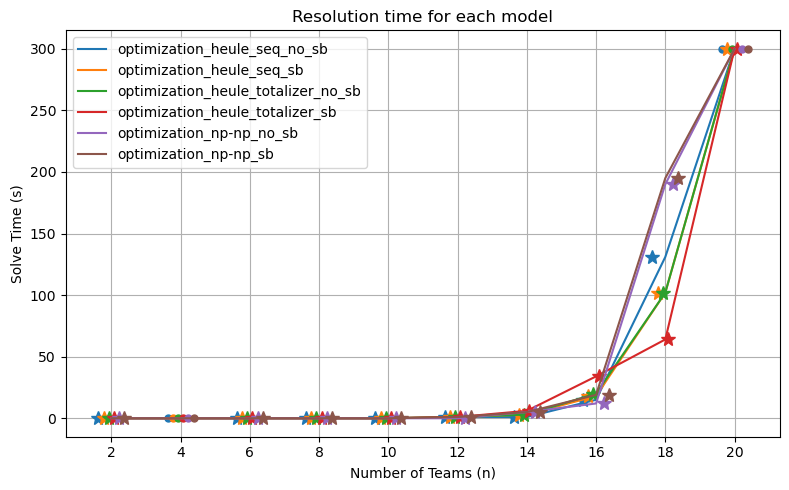
\includegraphics[width=\linewidth]{imgs/output.png}
        \caption{Resolution time}
    \end{subfigure}
    \caption{Runtimes for the optimization version of the Sports Tournament Scheduling (STS) problem. Data points are marked to indicate the solution status: a star ($\star$) indicates that a solution (optimal or sub-optimal) was found, while a circle ($\bullet$) indicates that no solution was found within the time limit.}
\end{figure}





\begin{thebibliography}{9}

\bibitem{dewerra1999}
Dominique de Werra.
\newblock Scheduling Round-Robin Tournaments: An Overview.
\newblock \emph{Discrete Applied Mathematics}, 91(1–3):241--277, 1999.

\bibitem{bailleux2003}
Olivier Bailleux and Yacine Boufkhad.
\newblock Efficient CNF Encoding of Boolean Cardinality Constraints.
\newblock In: \emph{Principles and Practice of Constraint Programming (CP 2003)}, Lecture Notes in Computer Science, 2003.
\end{thebibliography}

\end{document}
